\phantomsection
\part*{\textit{String Matching}}% -capitulo de string matching con ejemplos ilustrativos propios
% \addcontentsline{toc}{part}{String Matching}

\phantomsection
\section*{¿Qué es String Matching?}
% \addcontentsline{toc}{section}{¿Qué es String Matching?}

\quad String Matching es cuando se agarra un patrón y se buscan todas las instancias de ese patrón dentro de un texto específico. String es el término que se usan para las cadenas de texto y matching la palabra en inglés que dice que dos cosas concuerdan, en este caso la hilera del patrón con la hilera del texto.

\quad String Matching tiene varios usos en la vida real. Situaciones tan variadas como bases de datos musicales \maskCitep{FaroSimone2013Teos} y a la misma vez se puede usar para detección de plagio, forense digital, checkeo de palabras al escribir, detección de intrusión y muchísimos otros casos posibles (\cite{GeeksForGeekdsSM}). Para esta investigación nos vamos a basar en secuencias de ADN como uso del String Matching.

\phantomsection
\section*{Tipos de String Matching}
% \addcontentsline{toc}{section}{Tipos de String Matching}

\quad String Matching se subdivide en dos categorías: exactas y semejantes. Las dos de las categorías tienen sus propios algoritmos diferentes. En esta investigación no solo le daremos enfoque a la categoría de algoritmos de String Matching exactos, sino que nos vamos a analizar 4 algoritmos de este, los cuales serán: Fuerza Bruta (el más básico), Knuth-Morris-Pratt, Boyer-Moore y finalmente el Rabin-Karp. A cada uno se le va a dar un enfoque mayor en la siguiente parte de la investigación, pero en general lo que los destaca es que los primeros tres son con revisión de caracteres y el último utiliza hashing (que convierte uno o varios elementos de entrada a una función en otro elemento).

\section*{Ejemplo ilustrativo de String Matching}
\begin{figure} [H]
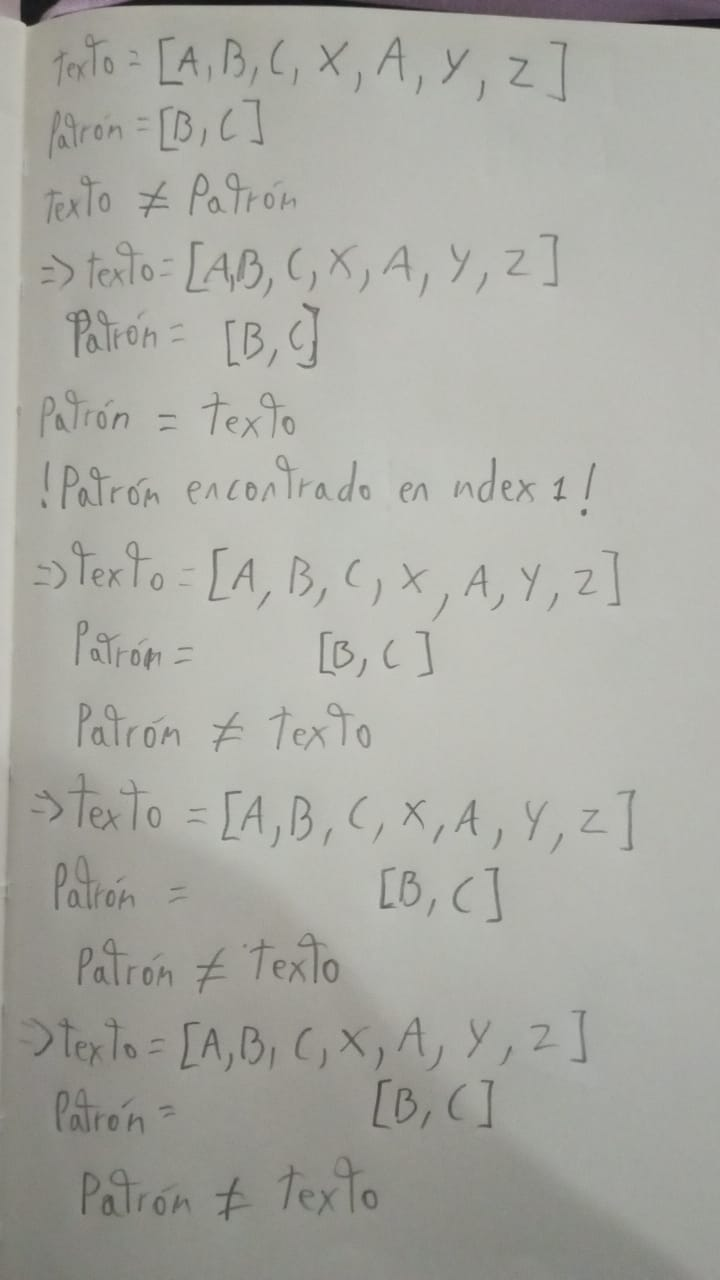
\includegraphics[width=0.5\textwidth]{WhatsApp_Image_2022-07-04_at_6.06.29_AM.jpeg}
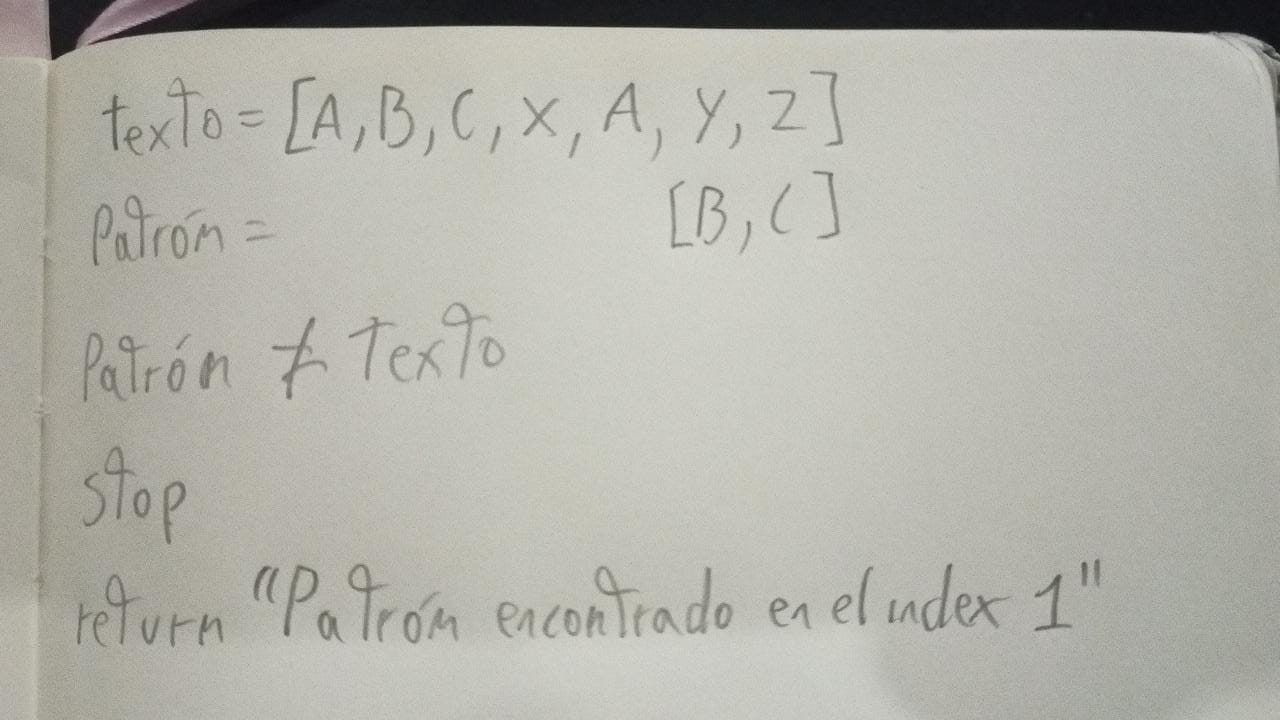
\includegraphics[width=0.5\textwidth]{WhatsApp_Image_2022-07-04_at_6.06.47_AM.jpeg}
\caption{Ilustrado}
\label{fig:Il}
\end{figure}
%codigo tikz buscado se puede implementar a una fecha mas tarde
% \def\nullvalue{}
% \def\drawarraystack(#1, #2, #3){
%   \begin{tikzpicture}
%     \def\scale{0.5}
%     \def\array{#1}
%     \def\top{#2}
%     \def\length{#3}
%     \foreach \i/\j in \array {
%       \node[minimum size=\scale cm] at (\i * \scale, \scale) (index\i) {\footnotesize \i};
%       \ifthenelse{\equal{\j}{\nullvalue}}{
%         \def\fillcolor{lightgray}
%       }{
%         \def\fillcolor{lightgray!40}
%       }
%       \node[draw, fill=\fillcolor, minimum size=\scale cm] at (\i * \scale, 0) {\j};
%     }
%     \fill [fill=lightgray] (\length * \scale + \scale * 0.5, 0 - \scale * 0.5) -- +(\scale, 0) -- +(\scale, \scale) -- +(0, \scale) -- cycle;
%     \draw (\length * \scale + \scale * 0.5, 0 - \scale * 0.5) -- +(\scale, 0);
%     \draw (\length * \scale + \scale * 0.5, 0 + \scale * 0.5) -- +(\scale, 0);
%     \node at (0, 0) (start) {\small $S$};
%     \node at (\top * \scale, 0) (top) {};
%     \node at (\top* \scale, -1) (pointer) {\small $S.top = \top$};
%     \draw [-{Stealth[sep=6pt]}] (pointer) -- (top);
%   \end{tikzpicture}
% }

% \begin{figure}[H]
%     \begin{tikzpicture}
%         \matrix (A) [matrix of nodes, nodes={draw, minimum size=10mm},
%             column sep=-\pgflinewidth]{
%             a & b & c & x & y & z & a & b & c\\};
%         \foreach \i [evaluate=\i as \ni using {int(\i)},
%                         evaluate=\i as \ntext using {int(\i-1)}] in {1,3,4,6} 
%             \draw [{Stealth}-, red!70] (A-1-\ni.south west)--++(-90:5mm) node[below] {\ntext};
%         \end{tikzpicture}
% \end{figure}

% \begin{tikzpicture}[font=\ttfamily,
%     array/.style={matrix of nodes,nodes={draw, minimum size=7mm, fill=green!30},column sep=-\pgflinewidth, row sep=0.5mm, nodes in empty cells,
%     row 1/.style={nodes={draw=none, fill=none, minimum size=5mm}},
%     row 1 column 1/.style={nodes={draw}}}]
    
%     \matrix[array] (array) {
%     0 & 1 & 2 & 3 & 4 & 5 & 6 & 7 & 8 & 9\\
%       &   &   &   &   &   &   &   &   &  \\};
%     \node[draw, fill=gray, minimum size=4mm] at (array-2-9) (box) {};
    
%     \begin{scope}[on background layer]
%     \fill[green!10] (array-1-1.north west) rectangle (array-1-10.south east);
%     \end{scope}
    
%     \draw[<->]([yshift=-3mm]array-2-1.south west) -- node[below] {Array length is 10} ([yshift=-3mm]array-2-10.south east);
    
%     \draw (array-1-1.north)--++(90:3mm) node [above] (first) {First index};
%     \draw (array-1-10.east)--++(0:3mm) node [right]{Indices};
%     \node [align=center, anchor=south] at (array-2-9.north west|-first.south) (8) {Element\\ (at index 8)};
%     \draw (8)--(box);
%     %
%     \end{tikzpicture}
